\documentclass{beamer}
\usetheme{uic}
\usepackage{amsfonts,amsmath,oldgerm,algorithmic,algorithm}
\usepackage[font=small,labelfont=bf]{caption} % Required for specifying captions to tables and figures

\newcommand{\hrefcol}[2]{\textcolor{uihteal}{\href{#1}{#2}}}
\newcommand{\testcolor}[1]{\colorbox{#1}{\textcolor{#1}{test}}~\texttt{#1}}

% Please see Section 18.1 of Beamer User Guide for all the options \usefonttheme provides
\usefonttheme[onlymath]{serif}
% \usefonttheme{serif} % use this if you would like Serif font throughout (and not just for math)

\title{Self-Introduction}
%\titlebackground{images/uic_halls.jpg}
% an asterisk will split the background:
% \titlebackground*{images/uic_seo.jpg}
\titlebackground*{images/About_Me.jpg}
%\subtitle{Using \LaTeX\ to prepare slides}

\author{\href{mailto:haozhang@me.com}{Hao ZHANG}}
\date{\today}

\begin{document}
	\maketitle
	
	% default is no footline, but page numbers are incredibly useful for the audience to ask questions later
	\footlinecolor{uicblue}
	
	\begin{frame}{About me...}
		My name is Hao ZHANG, I'm Chinese, I live in Paris now...
		\begin{itemize}
			\item In 2022, I completed my Specialized Master\textsuperscript{\textregistered}'s degree in SMART SYSTEMS \& IoT at CY Tech (formerly EISTI).
			\item Before pursuing this Specialized Masterr\textsuperscript{\textregistered}'s degree, I graduated from Leonardo da Vinci Engineering School (ESILV), specializing in Computer Science, Big Data and Connected Objects (IBO) in the Research path with the Data Science option.
			\item I have two different backgrounds...
		\end{itemize}
	\end{frame}
	
	\begin{chapter}[images/Formations.jpg]{steelgray}{Two different backgrounds}
	\end{chapter}
	
	\begin{frame}[fragile]{In the healthcare sector}
		\begin{itemize}[<+->]
			\item I was an undergraduate medical student.
			\item In 2009, after my bachelor's degree, I took part in an international program between China and France, so I had a chance to do some simple internships (more like an observer) at some hospitals in Paris.
			\item After my return, I worked in a Chinese pharmaceutical company, as a researcher in strategic analysis of the pharmaceutical industry.
		\end{itemize}
	\end{frame}
	
	\begin{frame}[fragile]{Why start learning data science?}
		\begin{itemize}[<+->]
			\item Because of my work during this period, I was exposed to a lot of data analysis work, and gradually built up a strong interest in this aspect.
			\item  I got advice from a respected industry leader.
			\item Last but not least, I see a huge opportunity for unification and potential synergy in healthcare with megadata technologies.
		\end{itemize}
	\end{frame}
	
	\begin{chapter}[images/Data_Lover.jpg]{uicblue}{The start of learning data science}
		\textit{Follow the trend and I'll go from there to further and further...}
	\end{chapter}
	\themecolor{light}
	
	\begin{frame}[fragile]{Learning data science and AI}
		\begin{itemize}[<+->]
			\item 2015 - 2017 University of Chongqing (CQU), Computer Technology Engineer
			\item 2017 - 2020 Leonardo da Vinci Engineering School (ESILV), Computer Science, Big Data and Connected Objects with the option in Data Science 
			\item 2020 - 2022 CY Tech (EISTI), Smart Systems \& Internet of Things 
		\end{itemize}
	\end{frame}
	
	\begin{frame}[fragile]{Internships in France}
		\begin{itemize}
			\item CSTB, Intern in the development of economic simulation programs in Python
			\begin{itemize}
				\item Development of a VBA economic simulation program using Python;
				\item Optimization of the program with vectorization to improve the speed and efficiency of calculations.
			\end{itemize}
			\item ELLIADD of UFC, Intern in ontology development and its semantic platform
			\begin{itemize}
				\item Development of an ontology and a graphical database (Neo4j) in the field of digital humanities;
				\item Development of intelligent services on a semantic platform based on an ontology-linked database.
			\end{itemize}
		\end{itemize}
	\end{frame}
	
	\begin{frame}[fragile]{My offline learning practices (1)}
		\begin{figure}[!htb]
			\minipage{0.2\textwidth}
			\endminipage\hfill
			\minipage{0.33\textwidth}
			\centering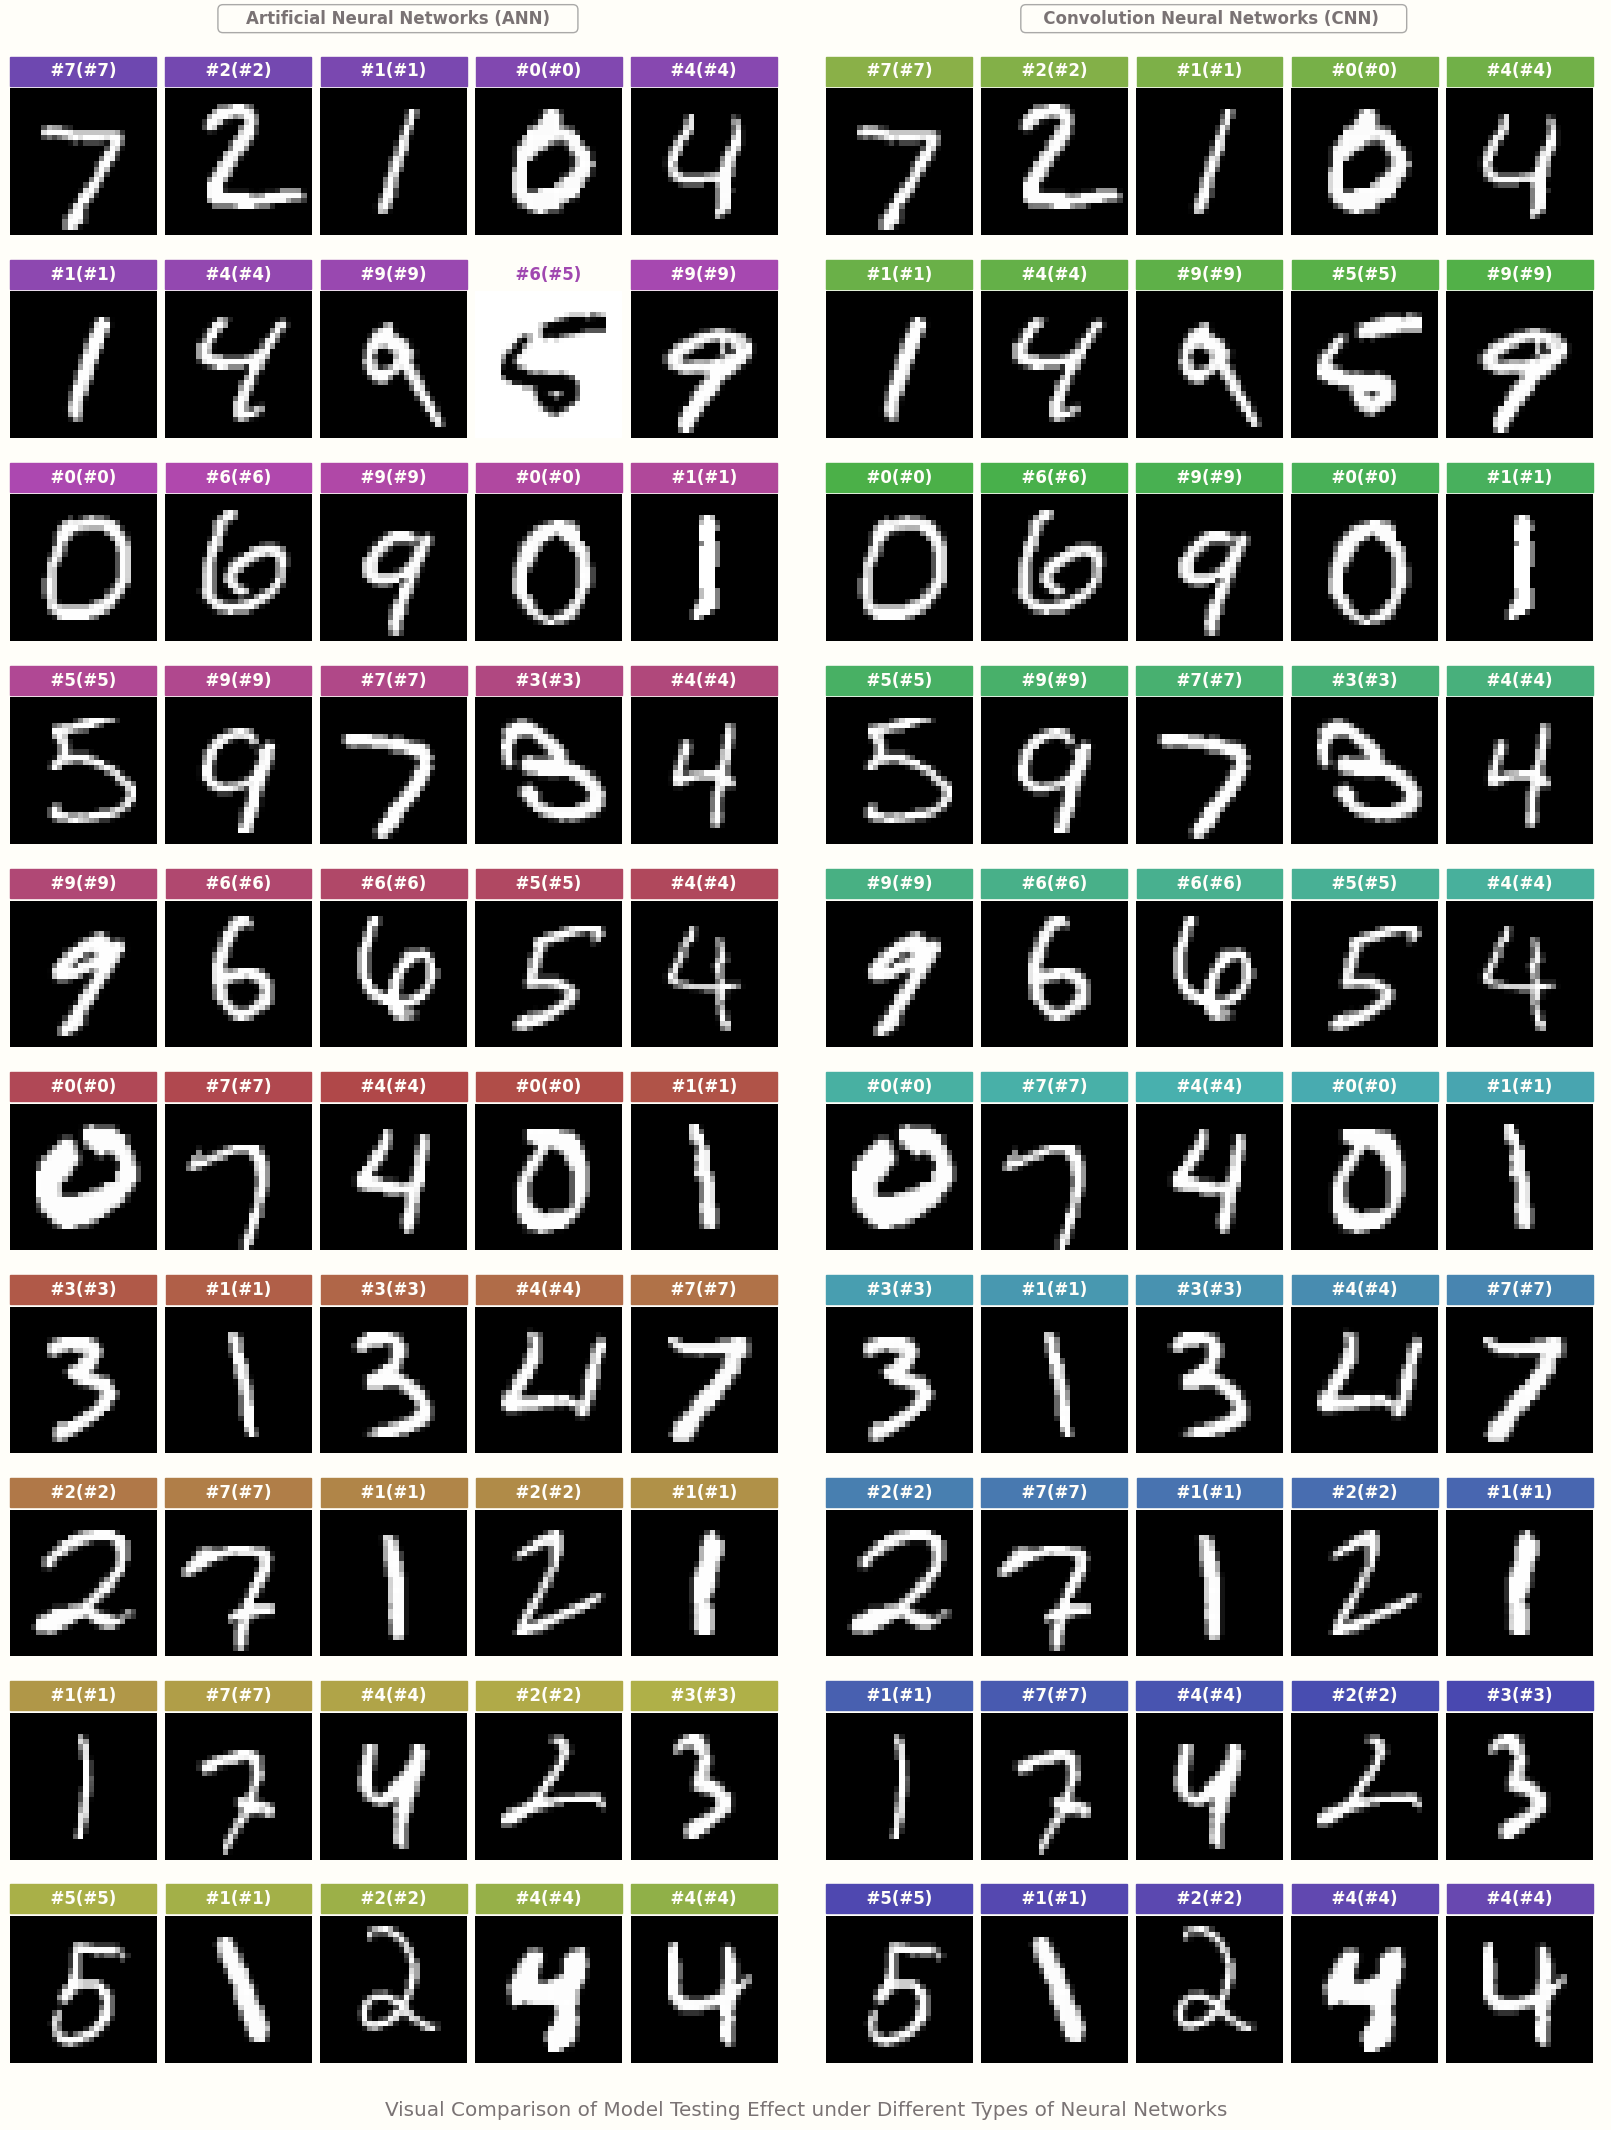
\includegraphics[width=\linewidth]{images/deep_learning_1.png}
			%\caption{A really Awesome Image}\label{fig:awesome_image1}
			\endminipage\hfill
			\minipage{0.33\textwidth}
			\centering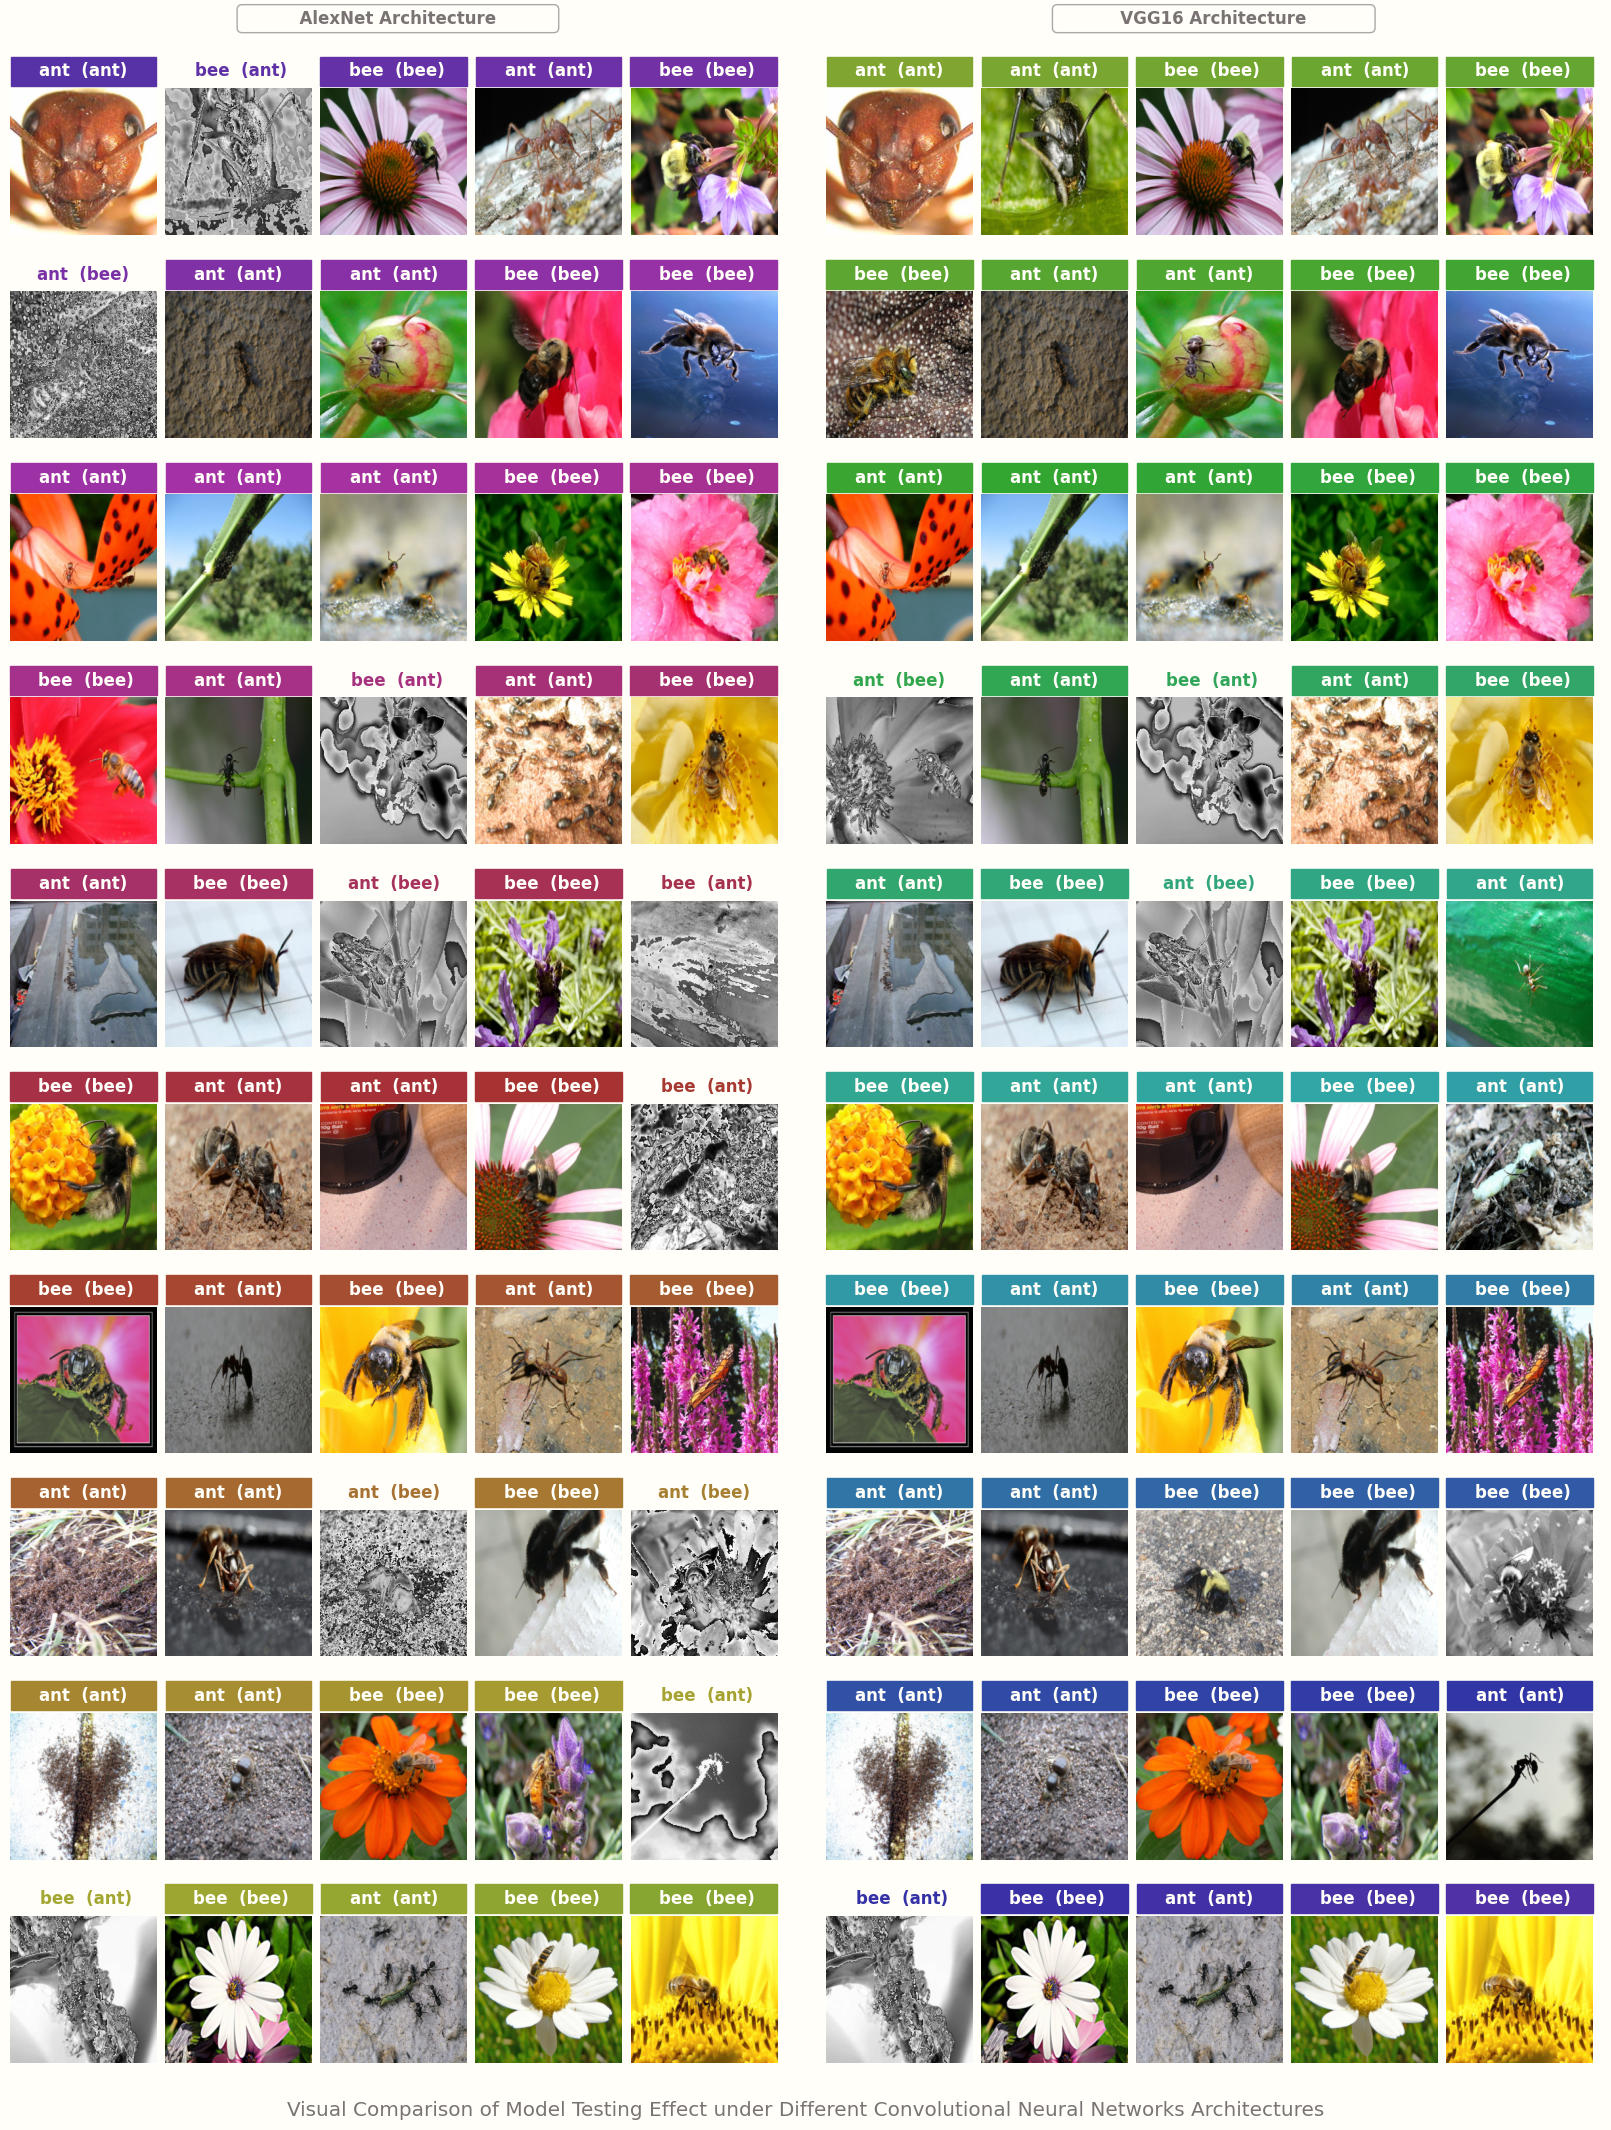
\includegraphics[width=\linewidth]{images/deep_learning_2.png}
			%\caption{A really Awesome Image}\label{fig:awesome_image2}
			\endminipage\hfill
			\minipage{0.14\textwidth}
			\rotatebox{270}{\normalfont\footnotesize{Learning\_Outcomes\_EN/}}
			\rotatebox{270}{\normalfont\footnotesize{Udemy\_Data\_Science\_Courses\_\\}}
			\rotatebox{270}{\normalfont\footnotesize{https://github.com/RaphaelZH/\\}}  
			\endminipage
		\end{figure}
	\end{frame}
	
	\begin{frame}[fragile]{My offline learning practices (2)}
		\begin{figure}[!htb]
			\minipage{0.55\textwidth}
			\centering\includegraphics[width=\linewidth]{images/deep_learning_3_1.png}
			%\caption{A really Awesome Image}\label{fig:awesome_image2}
			\endminipage\hfill
			\minipage{0.45\textwidth}
			\centering\includegraphics[width=\linewidth]{images/deep_learning_3_2.png}
			%\caption{A really Awesome Image}\label{fig:awesome_image1}
			\endminipage
		\end{figure}
		\vspace{-.4em}
		\begin{columns}
			\column{0.05\textwidth}
			\column{0.95\textwidth}
			\normalfont\footnotesize{https://github.com/RaphaelZH/Udemy\_Data\_Science\_Courses\_Learning\_Outcomes\_EN/}
		\end{columns}
	\end{frame}
	
	\begin{frame}[fragile]{My offline learning practices (3)}
		\begin{figure}[!htb]
			\vspace{-.25em}
			\minipage{0.34\textwidth}
			\centering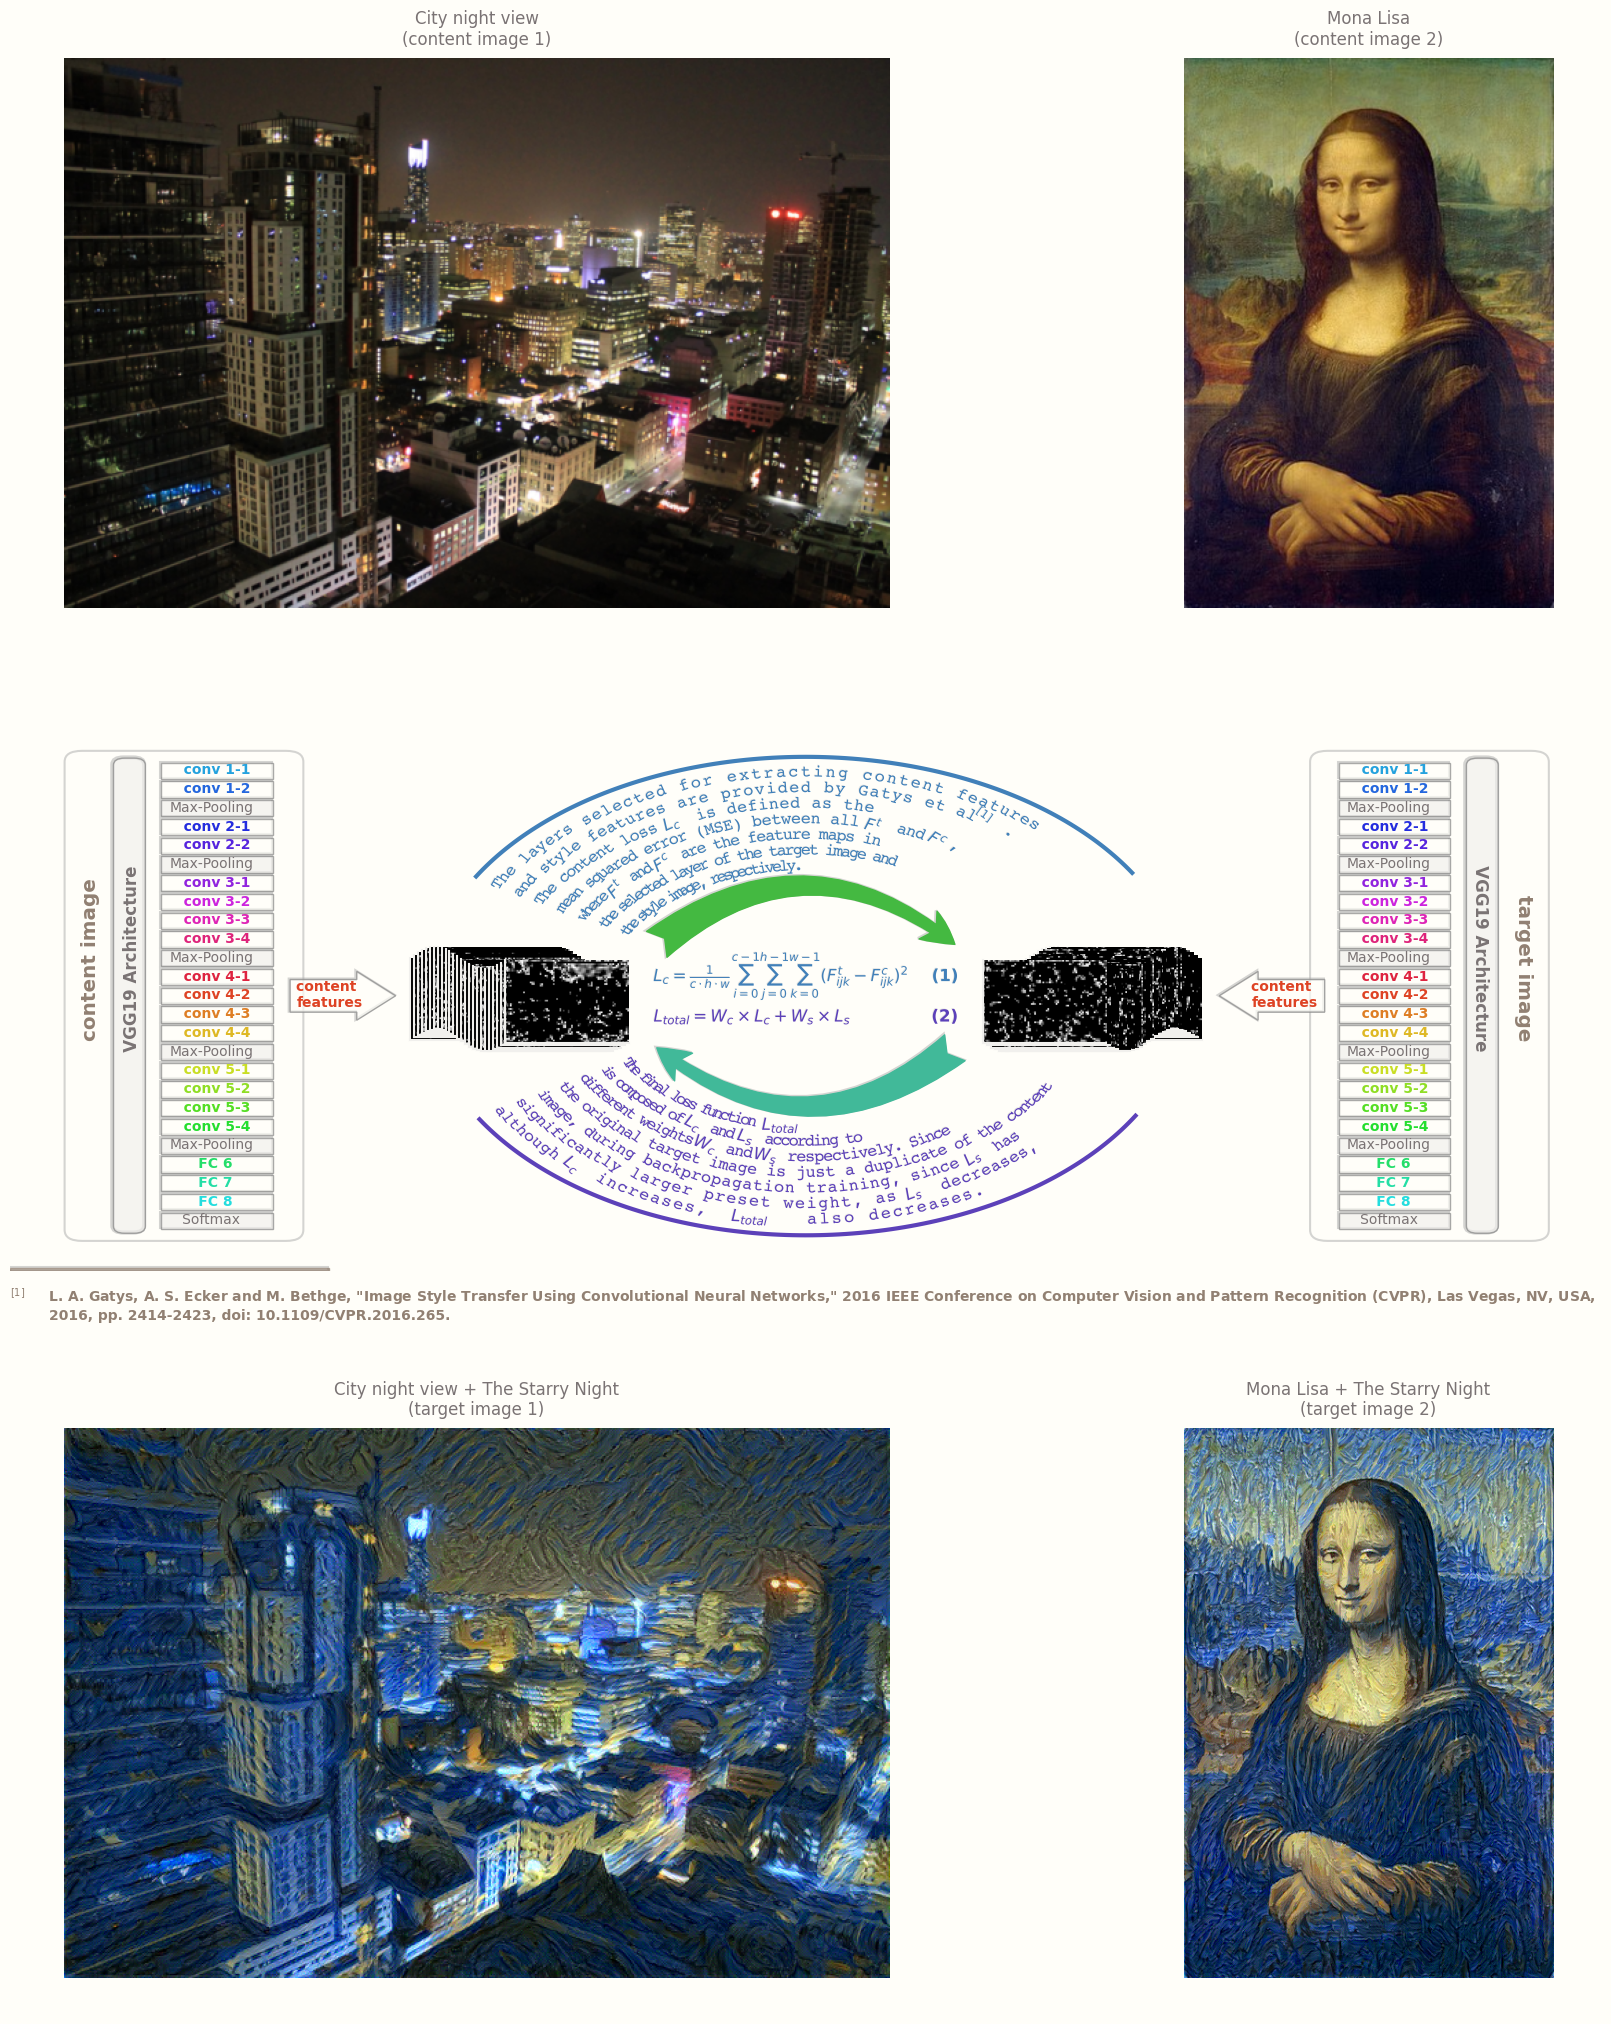
\includegraphics[width=\linewidth]{images/deep_learning_4_1.png}
			%\caption{A really Awesome Image}\label{fig:awesome_image2}
			\endminipage\hfill
			\minipage{0.43\textwidth}%
			\centering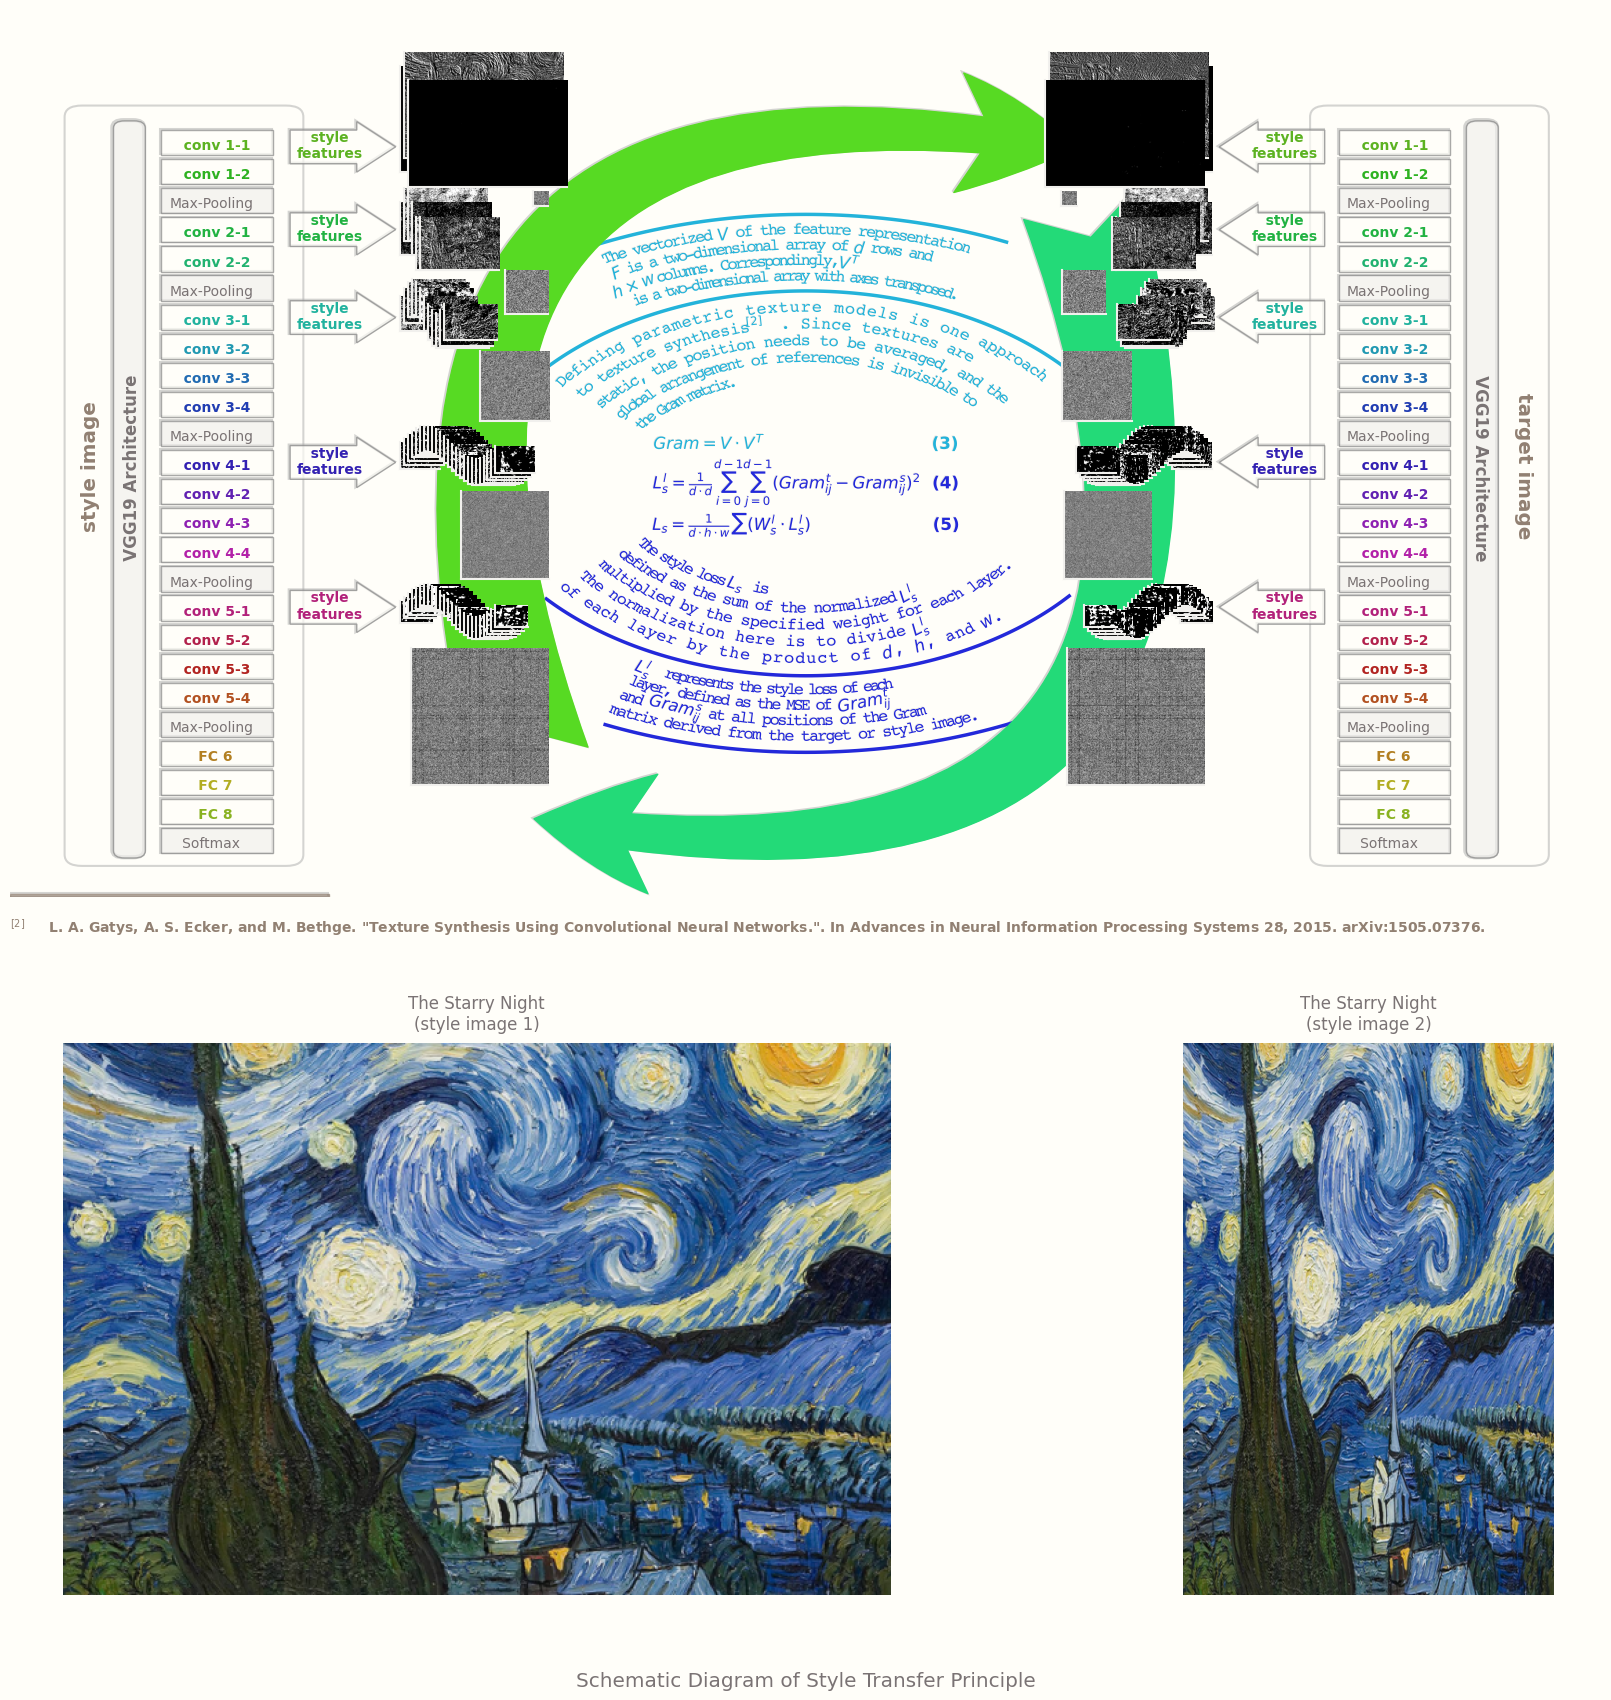
\includegraphics[width=\linewidth]{images/deep_learning_4_2.png}
			%\caption{A really Awesome Image}\label{fig:awesome_image3}
			\endminipage\hfill
			\minipage{0.1\textwidth}
			\rotatebox{270}{\normalfont\footnotesize{Learning\_Outcomes\_EN/}}
			\rotatebox{270}{\normalfont\footnotesize{Udemy\_Data\_Science\_Courses\_\\}}
			\rotatebox{270}{\normalfont\footnotesize{https://github.com/RaphaelZH/\\}}  
			\endminipage
		\end{figure}
	\end{frame}
	
	\begin{frame}[fragile]{My offline learning practices (4)}
		\begin{figure}[!htb]
			\vspace{-.25em}
			\minipage{0.33\textwidth}
			\centering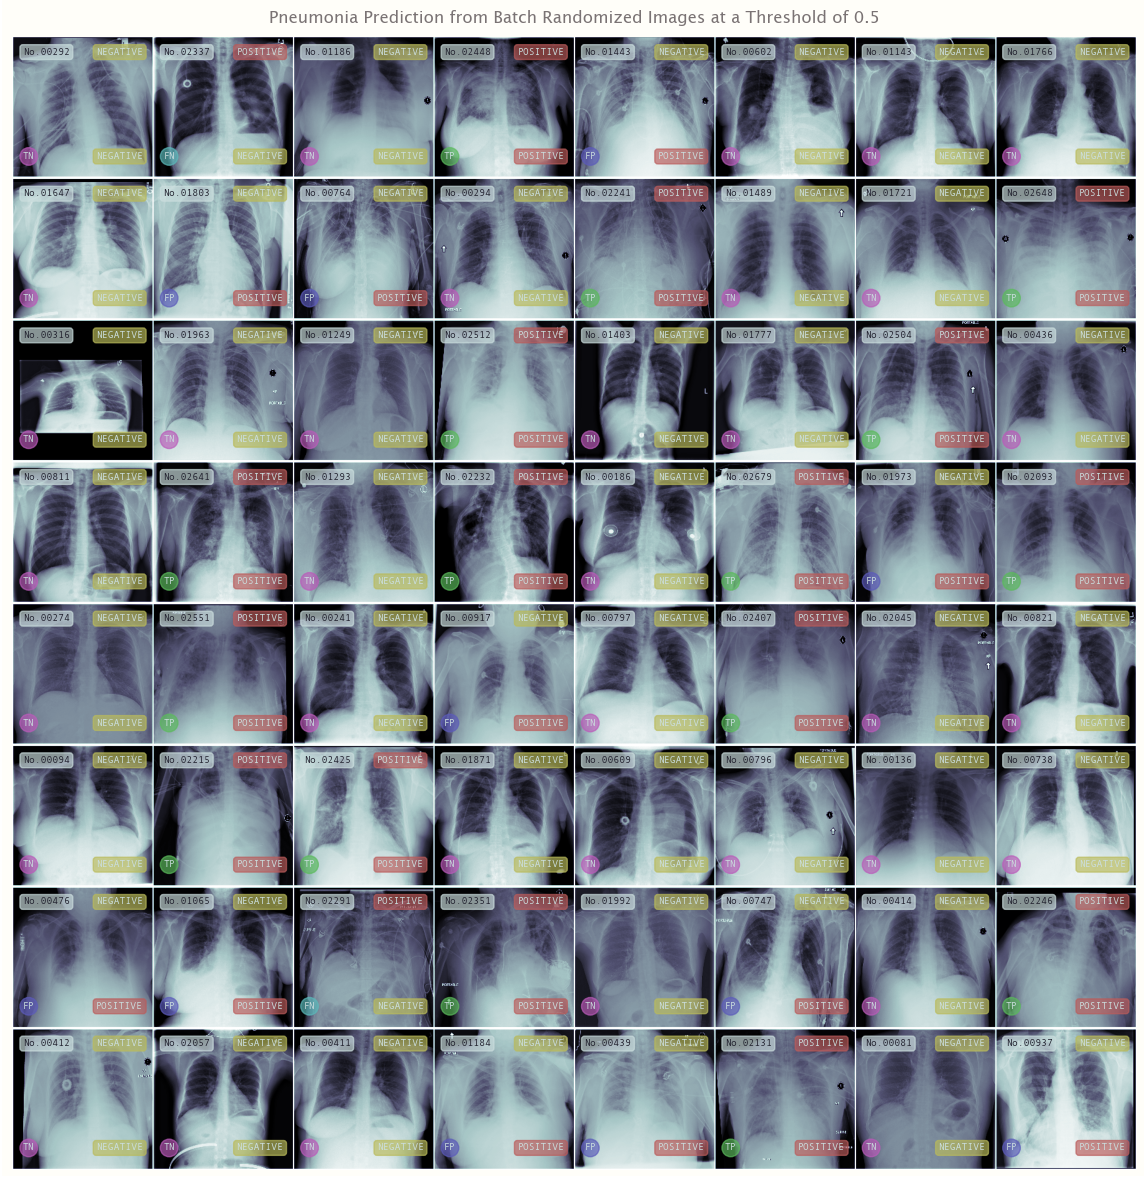
\includegraphics[width=\linewidth]{images/deep_learning_5_1_1.png}
			%\caption{A really Awesome Image}\label{fig:awesome_image2}
			\endminipage\hfill
			\minipage{0.33\textwidth}
			\centering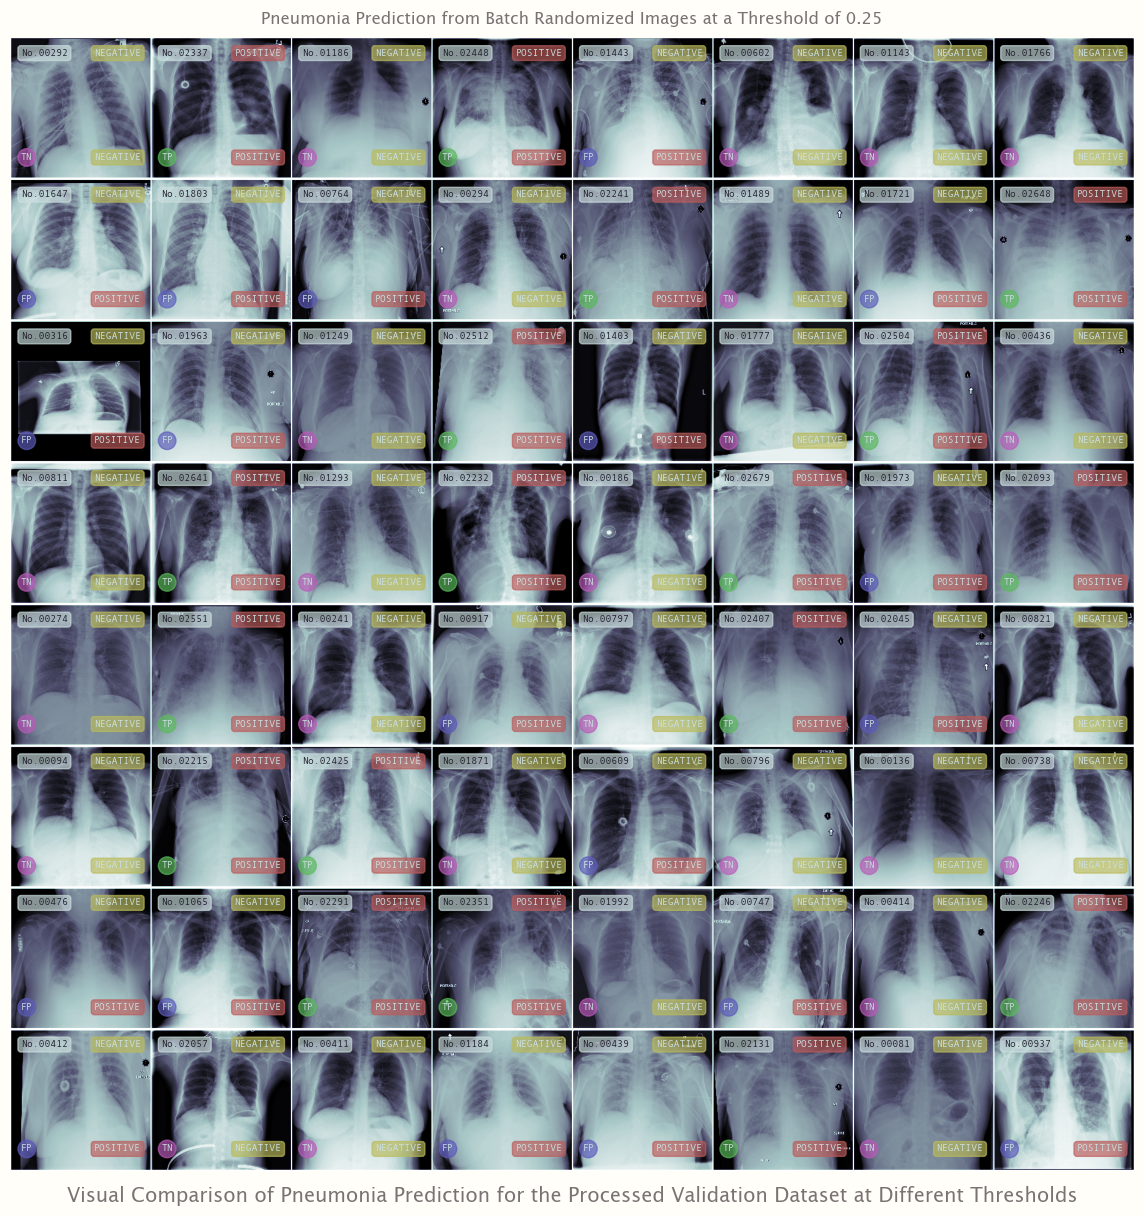
\includegraphics[width=\linewidth]{images/deep_learning_5_1_2.png}
			%\caption{A really Awesome Image}\label{fig:awesome_image2}
			\endminipage\hfill
			\minipage{0.3\textwidth}%
			\centering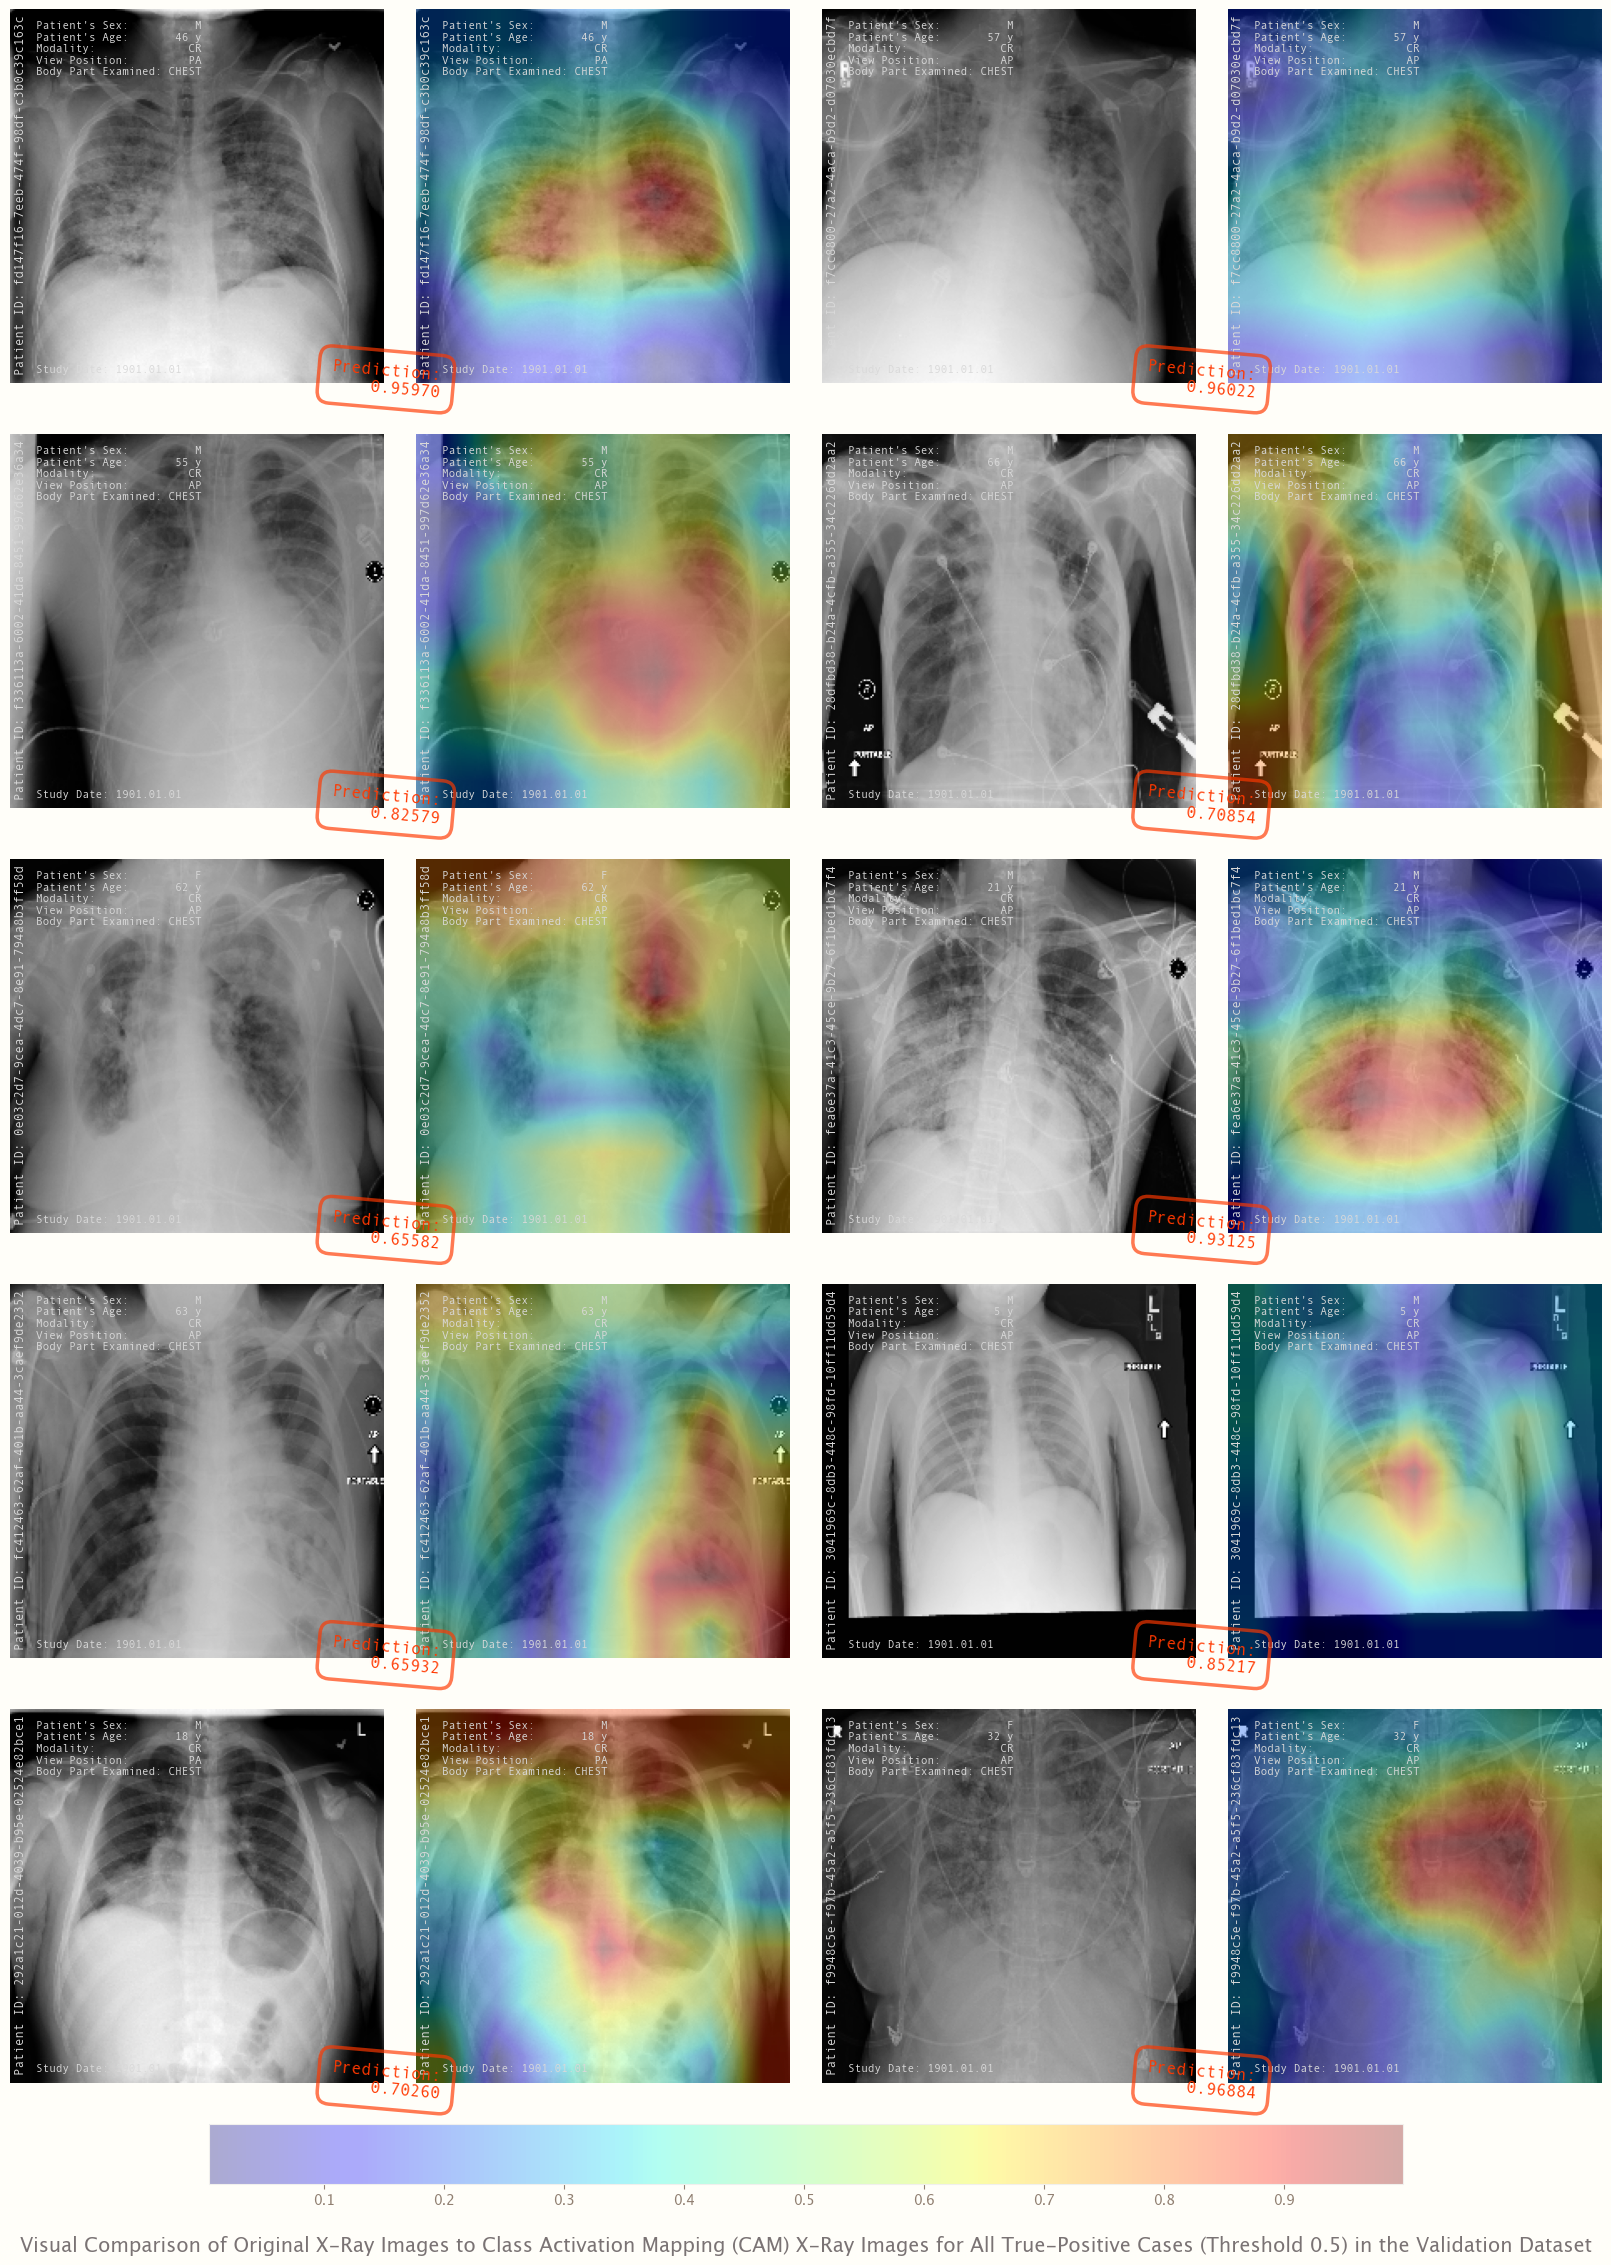
\includegraphics[width=\linewidth]{images/deep_learning_5_2.png}
			%\caption{A really Awesome Image}\label{fig:awesome_image3}
			\endminipage\hfill
			\vspace{.2em}
			\begin{columns}
				\column{0.05\textwidth}
				\column{0.95\textwidth}
				\normalfont\footnotesize{https://github.com/RaphaelZH/Udemy\_Data\_Science\_Courses\_Learning\_Outcomes\_EN/}
			\end{columns}
		\end{figure}
	\end{frame}
	
	\begin{frame}[fragile]{My offline learning practices (5)}
		\begin{figure}[!htb]
			\vspace{-.25em}
			\minipage{0.2\textwidth}
			\endminipage\hfill
			\minipage{0.4\textwidth}
			\centering\includegraphics[width=\linewidth]{images/deep_learning_6_1.png}
			%\caption{A really Awesome Image}\label{fig:awesome_image2}
			\endminipage\hfill
			\minipage{0.4\textwidth}%
			\centering\includegraphics[width=\linewidth]{images/deep_learning_6_2.png}
			%\caption{A really Awesome Image}\label{fig:awesome_image3}
			\endminipage\hfill
			\vspace{.2em}
			\begin{columns}
				\column{0.05\textwidth}
				\column{0.95\textwidth}
				\normalfont\footnotesize{https://github.com/RaphaelZH/Udemy\_Data\_Science\_Courses\_Learning\_Outcomes\_EN/}
			\end{columns}
		\end{figure}
	\end{frame}
	
	\begin{frame}[fragile]{My offline learning practices (6)}
		\begin{figure}[!htb]
			\vspace{-.25em}
			\minipage{0.0125\textwidth}
			\endminipage\hfill
			\minipage{0.225\textwidth}
			\centering\includegraphics[width=\linewidth]{images/deep_learning_7_1.png}
			\endminipage\hfill
			\minipage{0.025\textwidth}
			\endminipage\hfill
			\minipage{0.225\textwidth}
			\centering\includegraphics[width=\linewidth]{images/deep_learning_7_2.png}
			%\caption{A really Awesome Image}\label{fig:awesome_image2}
			\endminipage\hfill
			\minipage{0.025\textwidth}
			\endminipage\hfill
			\minipage{0.225\textwidth}%
			\centering\includegraphics[width=\linewidth]{images/deep_learning_7_3.png}
			\endminipage\hfill
			\minipage{0.025\textwidth}
			\endminipage\hfill
			\minipage{0.225\textwidth}%
			\centering\includegraphics[width=\linewidth]{images/deep_learning_7_4.png}
			%\caption{A really Awesome Image}\label{fig:awesome_image3}
			\endminipage\hfill
			\vspace{2em}
			\begin{columns}
				\column{0.05\textwidth}
				\column{0.95\textwidth}
				\normalfont\footnotesize{https://github.com/RaphaelZH/Udemy\_Data\_Science\_Courses\_Learning\_Outcomes\_EN/}
			\end{columns}
		\end{figure}
	\end{frame}
	
	\backmatter
\end{document}
